\subsection{Aplicación android}

Para realizar pruebas unitarias en android se utilizo la biblioteca JUnit la cual es utilizada para realizar pruebas unitarias en Java.

JUnit se utilizo sobre aquellas clases que se utilizaron para trabajar partes en especifico de la lógica del negocio que no involucraban utilitarias de android, es decir, que solamente utilizan Java.

\subsubsection{Pruebas sobre la clase DateFormater}

La clase DateFormater se utiliza en la aplicación para obtener fechas y presentarlas en un formato correcto en pantalla, así como pasar de una cadena de texto a un objeto de tipo Date, por lo cual las as pruebas realizadas sobre esta clase fueron tres.

\begin{enumerate}
	\item En la primera se valida que la conversión de una cadena de texto a un objeto de tipo Date se haga correctamente siempre y cuando se trate de una cadena valida.
	\item En la segunda prueba se valida que se pueda pasar de un tipo date a una cadena de texto y que el valor que se obtenga sea el mismo.
	\item En la ultima prueba se valida que se lance una excepción si el valor a convertir a una cadena de texto no es valido.
\end{enumerate}

El código utilizado en cada una de las pruebas es el siguiente.

\lstinputlisting[language=Java]{capitulo6/unitarias/codigo/DateFormaterTest.java}

En el código anterior, cada uno de los métodos anotados con @Test es una prueba a ejecutar, la forma en la que se valida que la ejecución sea correcta es con la linea de código correspondiente a Assert.assertEquals, la cual compara dos valores y los compara, en caso de ser iguales la prueba es exitosa en caso contrario la prueba ha fallado.

En la ultima prueba la anotación @Test tiene como parámetro una excepción a esperar, si la excepción se dispara la prueba es correcta, por otro lado,  si no se da el caso la prueba ha fallado.

La correcta ejecución de las pruebas se puede apreciar en la figura \ref{fig:dateTest}.

\begin{figure}[h]
	\centering
	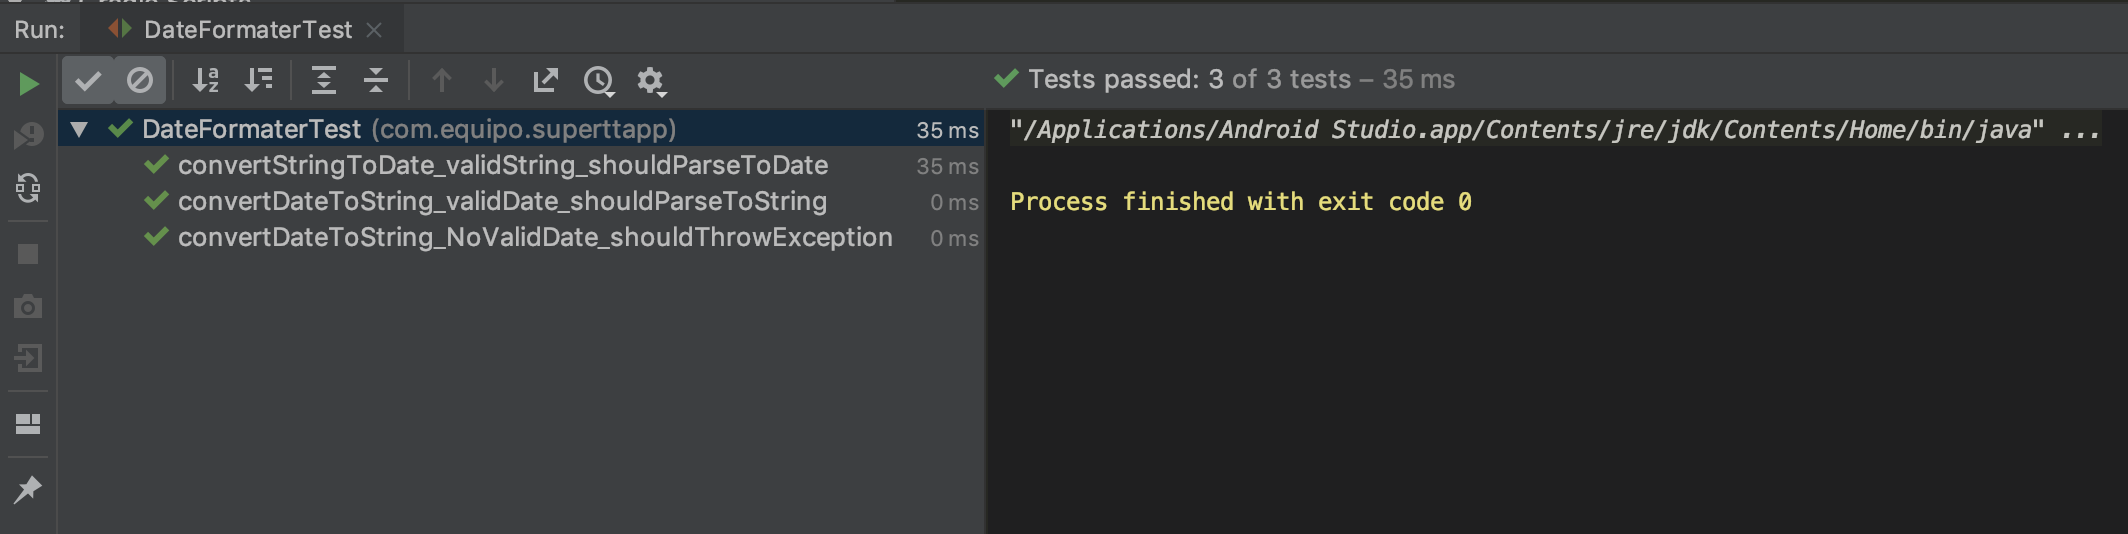
\includegraphics[width=450px]{capitulo6/unitarias/img/dateTest.png}
	\caption{Resultados de las pruebas de la clase DateFormater}
	\label{fig:dateTest}
\end{figure}

\subsubsection{Pruebas sobre la clase RNN002}
La clase RNN002 se utiliza en la aplicación para validar el formato de diversos campos que se tienen en los diferentes formularios que incluye la aplicación, es por esto que las pruebas que se realizaron en este caso fueron las siguientes.

\begin{enumerate}
	\item En la primera prueba se verifica que para un email valido, el resultado sea true.
	\item En la siguiente prueba, para un email no valido, el resultado debe de ser false.
	\item En la siguiente prueba, para una contraseña valida, el resultado debe de ser true.
	\item En la siguiente prueba, para una contraseña no valida, el resultado debe de ser false.
	\item En la siguiente prueba, para dos contraseñas validas, el resultado debe de ser true.
	\item En la siguiente prueba, para dos contraseñas, una de ellas no valida, el resultado debe de ser false.
	\item En la siguiente prueba, para un nombre valido, el resultado debe de ser true.
	\item En la siguiente prueba, para un nombre no valido, el resultado debe de ser false.
	\item En la siguiente prueba, para un apellido valido, el resultado debe de ser true.
	\item En la siguiente prueba, para un apellido no valido, el resultado debe de ser false.
	\item En la siguiente prueba, para un nombre de proyecto valido, el resultado debe de ser true.
	\item En la ultima prueba, para un nombre de proyecto no valido, el resultado debe de ser false.
\end{enumerate}

El código utilizado en cada una de las pruebas es el siguiente.

\lstinputlisting[language=Java]{capitulo6/unitarias/codigo/RN002Test.java}

En el caso de estas pruebas presentadas en el código anterior, se utilizaron los métodos Assert.assertTrue y Assert.assertFalse para verificar que las pruebas fueran correctas. En el caso del primero de estos métodos la prueba es exitosa si el valor que retorna el método a probar es falso, mientras que para el segundo método si el valor de retorno es falso la prueba es correcta.

La ejecución de las pruebas se muestra en la figura \ref{fig:rnn002Test}.

\begin{figure}[h]
	\centering
	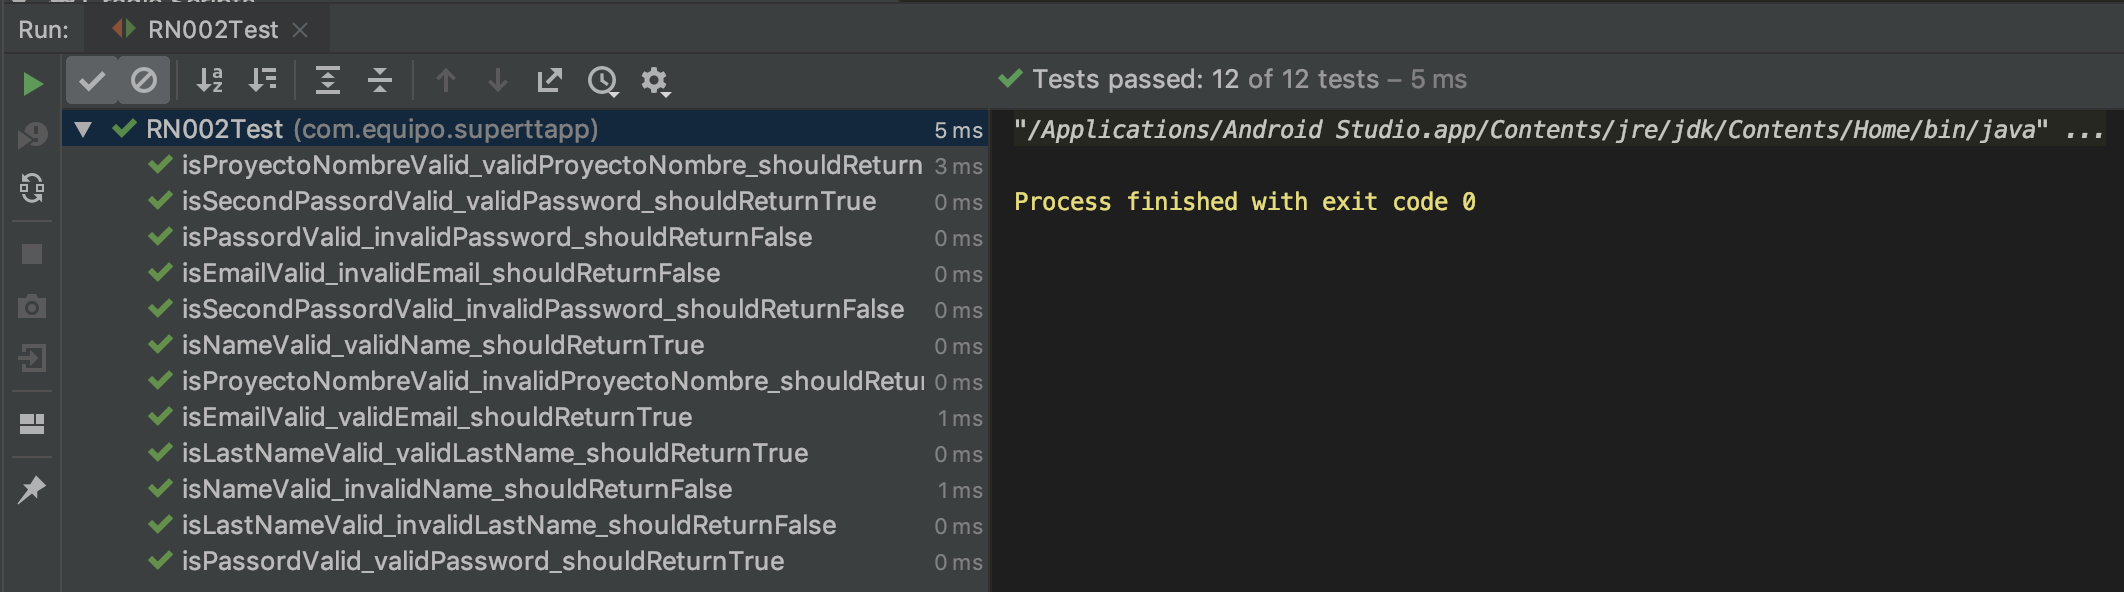
\includegraphics[width=450px]{capitulo6/unitarias/img/rnn002Test.png}
	\caption{Resultados de las pruebas de la clase RNN002}
	\label{fig:rnn002Test}
\end{figure}